\section{Theorie}
\label{sec:theorie}
Die Theorie bezieht sich für die Kathodenstrahlröhre und elektrische Felder
auf \cite{Anleitung501}, für das Magnetfeld auf \cite{Anleitung502}.
\subsection{Kathodenstrahlröhre}
In der benutzten Kathodenstrahlröhre werden die Elektronen mittels des Effekts
aus V504 - Thermische Elektronenemission - mit einer indirekten Heizung aus der
Kathode gelöst.
Mittels eines Wehneltzylinders und verschiedenen Elektroden wird der Strahl
fokussiert und die einzelnen Elektronen beschleunigt.
Dies ist in Abbildung \ref{fig:kathstrahl} zu sehen. Mit zwei weiteren,
zueinander orthogonal ausgerichteten, Plattenpaaren kann der Strahl abgelenkt werden.
Die Röhre ist bis auf einen Restdruck von $p=\SI{e-6}{\milli\bar}$ evakuiert,
damit die Elektronen erst auf dem Schirm wechselwirken.

\begin{figure}
  \centering
  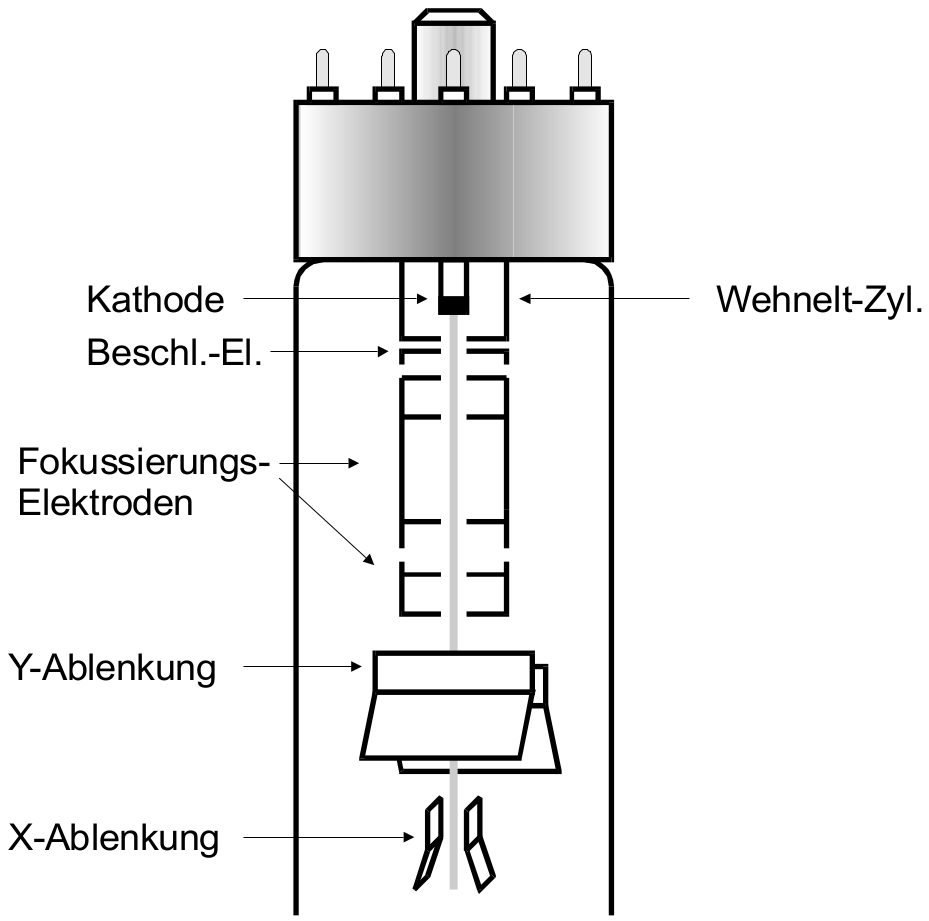
\includegraphics[width=7cm]{content/kathodenstrahl2.png}
  \caption{Schematischer Aufbau einer Kathodenstrahlröhre, aus \cite{Anleitung501}.}
  \label{fig:kathstrahl}
\end{figure}

\subsection{Elektronen im Elektrischen Feld}
Zwischen den Ablenkplatten, mit dem Abstand $d$ und der Länge $p$,
liegt eine Spannung $U_d$ an, die ein homogenes Feld in diesem Bereich erzeugt.
Die elektrische Kraft
\begin{equation}
      \left|\vec{F}\,\right| = \left|\,\symup{e}_0\vec{E}\,\right| = \symup{e}_0\frac{U_d}{d}
\end{equation}
fürht zu einer linearen Beschleunigung, z.B. in y-Richtung.
Nach Durchlaufen der Strecke $L$ zwischen Ablenkpunkt und Schirm ergibt sich
für die Auslenkung
\begin{equation}
      D = \frac{p}{2d}L\frac{U_d}{U_b}\:.
      \label{eqn:ablenkunge}
\end{equation}

\subsection{Kathodenstrahl-Oszillograph}
Eine Kathodenstrahlröhre kann als Oszillograph verwendet werden, wenn in einer
Ablenkrichtung eine Sägezahnspannung angelgt wird und in der anderen das zu untersuchende Signal.
Stehen die Frequenzen der Sägezahnspannung und z.B. einer Sinuswelle
im Verhältnis
\begin{equation}
      n\,ν_\text{sä} = m\,ν_\text{sin}\:,\;\;n,m \in \symbb{N}
      \label{eqn:frequenz}
\end{equation}

\subsection{Elektronen im Magnetfeld}
Die wirkende Kraft auf ein Elektron im Magnetfeld ist die Lorentzkraft
\begin{equation}
      \vec{F_\text{L}}= - \symup{e}_0\,\vec{v} \times \vec{B}\:.
\end{equation}
Bei senkrecht stehendem Magnetfeld ist die Kraft folglich am größten.
Im Gegensatz zum Elektrischen Feld wirkt das Magnetfeld auf der gesamten Länge
der Kathondenstrahlröhre. Die Elektronen bewegen sich aufgrund der linearen
Querbeschleunigung in einer Kreisbahn mit Radius
\begin{equation}
      r = \frac{\symup{m}_0 v_0}{\symup{e}_0 B}\:,
\end{equation}
dies folgt aus dem Gleichgewicht von Lorentz- und Zentrifugalkraft.
$v_0$ kann mit kinetischer und elektrischer Energie aus der Beschleunigungsspannung
$U_\text{B}$ nach
\begin{equation}
      v_0 = \sqrt{2 U_\text{B}\frac{\symup{e}_0}{\symup{m}_0}\,}
\end{equation}
bestimmt werden. Mit der Ablenkung $D$ auf dem Schirm vom feldfreien Auftreffpunkt
kann durch den Satz von Pythagoras die Formel
\begin{equation}
      \frac{D}{L^2+D^2} = \frac{1}{\sqrt{8 U_\text{B}}} \sqrt{\frac{\symup{e}_0}{\symup{m}_0}} B
      \label{eqn:ablenkungm}
\end{equation}
hergeleitet werden.
\\~\\
Der Betrag des Magnetfeldes der verwendeten Helmholtzspulen kann über
\begin{equation}
      B = μ_0 \frac{8}{\sqrt{125}} \frac{N I}{R}\:,
      \label{eqn:helmholtz}
\end{equation}
mit Windungszahl $N$, Radius $R$ und Strom $I$ berechnet werden.
